% Dokumentation af converter topologi

\chapter{Første Iteration}
I dette afsnit beskrives den indledende og første iteration af designfasen. Den indebære valg af converter topologi, samt simulering af en ideel converter.

\section{Switch Mode Power-Supply}
I dette projekt vælges der at tage udgangspunkt i Switch Mode Power-Supply (SMPS). Da der er stillet et krav om et maksimalt tab på 5W, betyder det, ved en maksimal udgangseffekt på 75W, at converteren skal have en effektivitet på:
\begin{equation}
	\eta = \frac{75W}{75W + 5W} \cdot 100 = 93.75
\end{equation}

En lineær converter vil ikke kunne opnå så stor en effektivitet. Denne effektivitet kan til gengæld tilnærmes ved brug af en SMPS. Det vælges at tage udgangspunkt i en flyback converter, da denne er ideel til effekter under 100W. 

%TODO find kilder der bekræfter disse påstande.

\section{Flyback Converter}
Flyback converteren, er en transformator baseret topologi. Man deler converteren op i to dele: Primær- og sekundærsiden. Primærsiden består af primærviklingen af transformatoren og en transistor, hvor transistoren fungerer som en switch. Sekundærsiden består af sekundærviklingen, en diode, en udgangskondesator og belastningen. Dette er vist på figur~\ref{fig:flyback_ideal}. En af fordelene ved at bruge flyback converteren er at der kan opnås galvanisk adskillelse mellem primær- og sekundærsiden af transformatoren. Derudover bruges der relativt få komponenter.

\begin{figure}[H]
	\center
	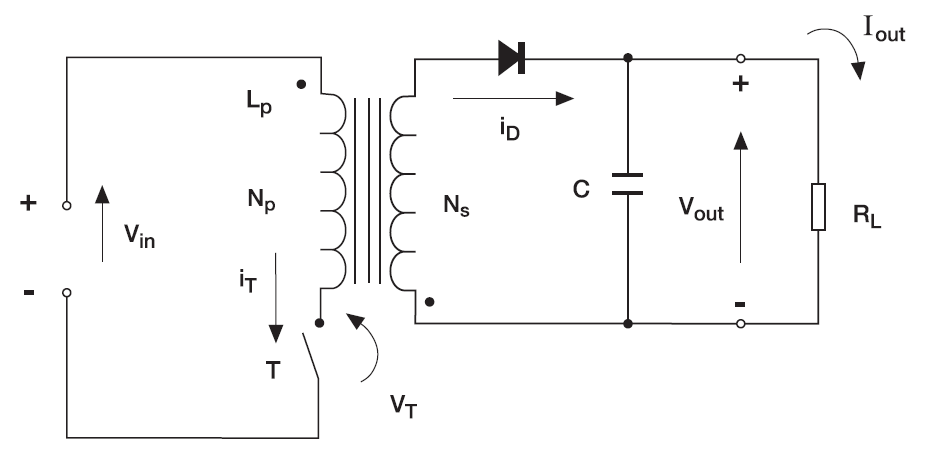
\includegraphics[max width=0.7\linewidth]{/tex/smps/billeder/flyback_ideal.PNG}
	\caption{Ideelt diagram af flyback converteren
	\cite{SMPS-topologies}}
	\label{fig:flyback_ideal}
\end{figure} 

Flyback converteren bruges til at konvertere en indgangsspænding, ned til en mindre udgangsspænding. Dette gøres ved at styre transistoren med et PWM-signal, med en variabel duty-cycle. Når den er ON, vil der være en positiv spænding ved prik-enden af viklingen ift. den anden ende. Ud fra formlen $V=L\cdot \frac{di}{dt}$ kan det ses, at når der ligger en spænding over viklingen, vil strømmen i transformatoren stige lineært, over den tid transistoren er ON. Når transistoren går OFF, vil den magnetiske strøm i transformatoren inducere en spænding over sekundærviklingen. Når denne spænding bliver lig udgangsspændingen, vil dioden begynde at lede den strøm, der er oplagret i transformatoren. Da spændingen over sekundærviklingen er positiv ved prikken, og dermed modsat af primærviklingen, vil strømmen falde lineært ud fra samme forhold, som nævnt tidligere. Dette vil over tid skabe en trekantet kurveform af den samlede strøm i transformatoren. Et eksempel på dette kan ses på figur \ref{fig:CCM_transformer_current}. Da strømmen i hver vikling er diskontinuert, vil det give anledning til større peak-strømme. Det er maksimalt $50\percent$ af tiden der løber en strøm i viklingen, hvilket betyder en større strøm for at opretholde den samme middelstrøm.

Flyback converteren kan overordnet drives på to forskellige måder, Continuous Conduction Mode (CCM) og Discontinuous Conduction Mode (DCM). Disse to måder har forskellige fordele og ulemper, som skal tages højde for inden der vælges hvordan converteren skal drives. 

\subsection{Continuous Conduction Mode}
Forkellen ved CCM og DCM er, hvordan strømmen løber i transformatoren. Ved CCM vil der altid løbe en strøm i transformatoren, som der også ligger i navnet. Dog vil strømmene individuelt i viklingerne være diskontinuerte. Strømmen er skitseret på figur \ref{fig:CCM_transformer_current}. Skal man have den samlede strøm i transformatoren, skal de to kurver for primær- og sekundærviklingen samles. Dette er fordi der kun løber en strøm i primærviklingen når transistoren er ON, og en strøm i sekundærviklingen når transistoren er OFF. 

\begin{figure}[H]
	\center
	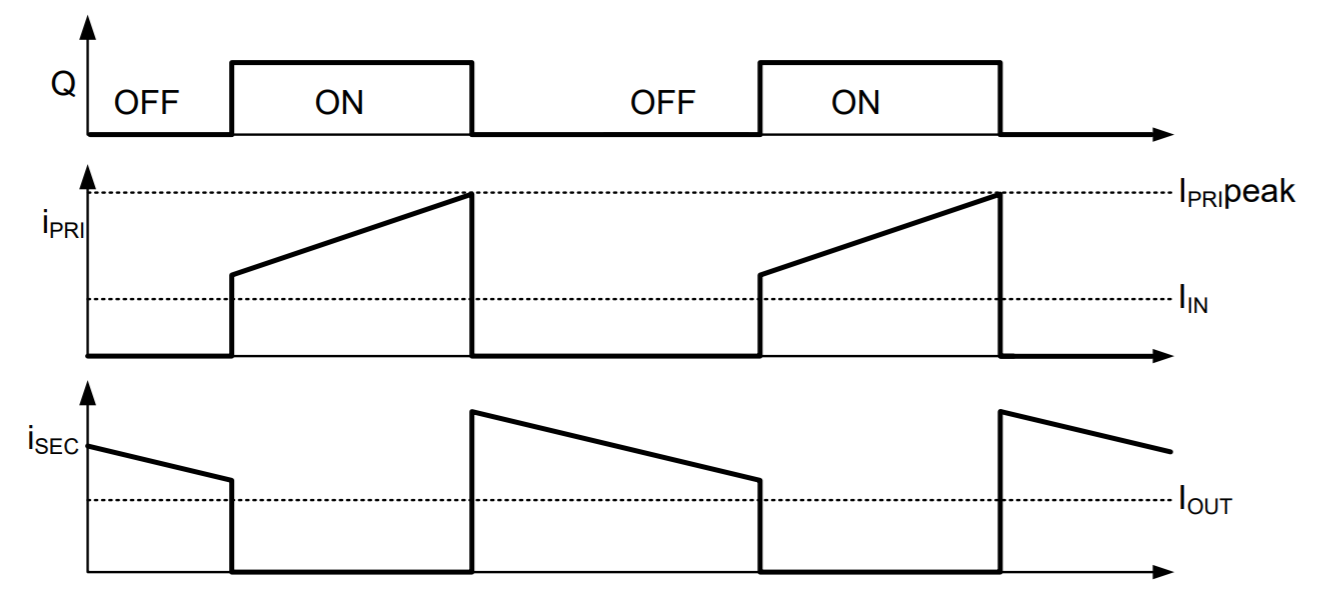
\includegraphics[max width=0.7\linewidth]{/tex/smps/billeder/CCM_transformer_current.PNG}
	\caption{CCM transformator strømme}
	%\cite{SMPS-topologies}}
	\label{fig:CCM_transformer_current}
\end{figure}

\noindent En af fordelene ved CCM er, at strømmen i transformatoren ikke når at aflade helt, inden transistoren går ON igen. Dette giver lavere ripple-strømme, og dermed også peak-strømme, hvilket giver anledning til et mindre effekttab. På grund af den mindre ripple-strøm i transformatoren, opnås der også en mindre ripplespænding på udgangen. hvilket sætter et mindre krav til udgangskondensatoren. 

\subsection{Discontinuous Conduction Mode}
Den anden måde at drive converteren på er DCM. Ved denne metode vil der være en død tid i hver periode, hvor der ikke løber en strøm i transformatoren. Dette betyder at transformatoren når at aflade helt, inden switch-perioden er ovre. Til forskel fra CCM, vil dette give nogle trekantede strømkurver i transformatoren, som ses på figur %TODO indsæt figur.
På grund af død tiden, vil peak-strømmene blive større, da arealet under kurven skal være det samme som ved DCM. fordelen ved at $di$ bliver større, er at induktansen i viklingerne bliver mindre. 

\section{Ideel transformator}
Der vælges at arbejde videre med en flyback converter i CCM, pga. kravet om et tab på maksimalt 5W. På grund af de store strømme i transformatorens viklinger, vurderes det at tabet i MOSFET og diode, vil være for stort når de leder. 

Det startes med at designe en converter der, ved en input spænding på $26V-100V$, kan opretholde en udgangsspænding på $21V$ og $2.5A$. 

\noindent Ud fra dette beregnes en maksimal og minimal duty-cycle:
\begin{equation} \label{D_maks_CCM}
D_{maks} = \frac{V_{out}}{V_{inmin} + V_{out}} = 0.447
\end{equation}
\begin{equation} \label{D_min_CCM}
D_{min} = \frac{V_{out}}{V_{inmaks} + V_{out}} = 0.174
\end{equation}

\noindent Nu kan de maksimale ripple-, peak- og RMS-strømme i transformatoren estimeres: 
\begin{equation} \label{I_ripple_CCM}
I_{ripple} = 0.6 \cdot \frac{V_{out} \cdot I_{out}}{V_{inmaks} \cdot   D_{min}} = 1.8A
\end{equation}
\begin{equation} \label{I_pk_CCM}
I_{pk} = \frac{V_{out} \cdot I_{out}}{V_{inmin} \cdot D_{maks}} + \frac{I_{ripple}}{2} = 5.4A
\end{equation}
\begin{equation} \label{I_pk_avg_CCM}
I_{pkavg} = \frac{I_{out}}{1-D_{maks}} = 4.5A
\end{equation}

\noindent Nu beregnes RMS-strømmene i både primær- og sekundærviklingerne. 
\begin{equation} \label{I_p_RMS_CCM}
I_{RMSp} = \sqrt{D_{maks} \cdot (I_{pkavg})^2} = 3A
\end{equation}
\begin{equation} \label{I_s_RMS_CCM}
I_{RMSs} = \sqrt{(1-D_{maks}) \cdot (I_{pkavg})^2} = 3.4A
\end{equation}

Induktansen i primærviklingen beregnes ud fra den ønskede ripplestrøm, samt switch-frekvensen. Som udgangspunkt vælges den til $100kHz$. Derudover vælges det, at have et omsætningsforhold lig 1 i transformatoren, hvilket betyder $L_p = L_s$.
\begin{equation} \label{L}
L = \frac{V_{inmin} \cdot D_{min}}{I_{ripple} \cdot f_s} = 95.6\micro H
\end{equation}



\section{Udgangskondensator}
I en flyback converter bruges udgangskondensatoren primært til at mindske ripplespændingen på load'en. Formlen for at beregne minimumskapaciteten er
\begin{equation} \label{udgangskondensator}
C_{out} \geqslant \frac{I_{out} \cdot D_{max}}{V_{ripple} \cdot f_s} \geqslant 223.4 \micro F
\end{equation}

\section{Simulering}
Med udgangspunkt i figur~\ref{fig:flyback_ideal} opsættes en ideel flyback converter i p-spice. Dette er gjort på figur~\ref{fig:ideal_flyback_diagram}. Converteren er sat op med en ideel transformatorkobling, et ideelt switching element, samt en ideel diode, for at få et indblik i flyback converterens virkemåde. 


\begin{figure}[H]
	\center
	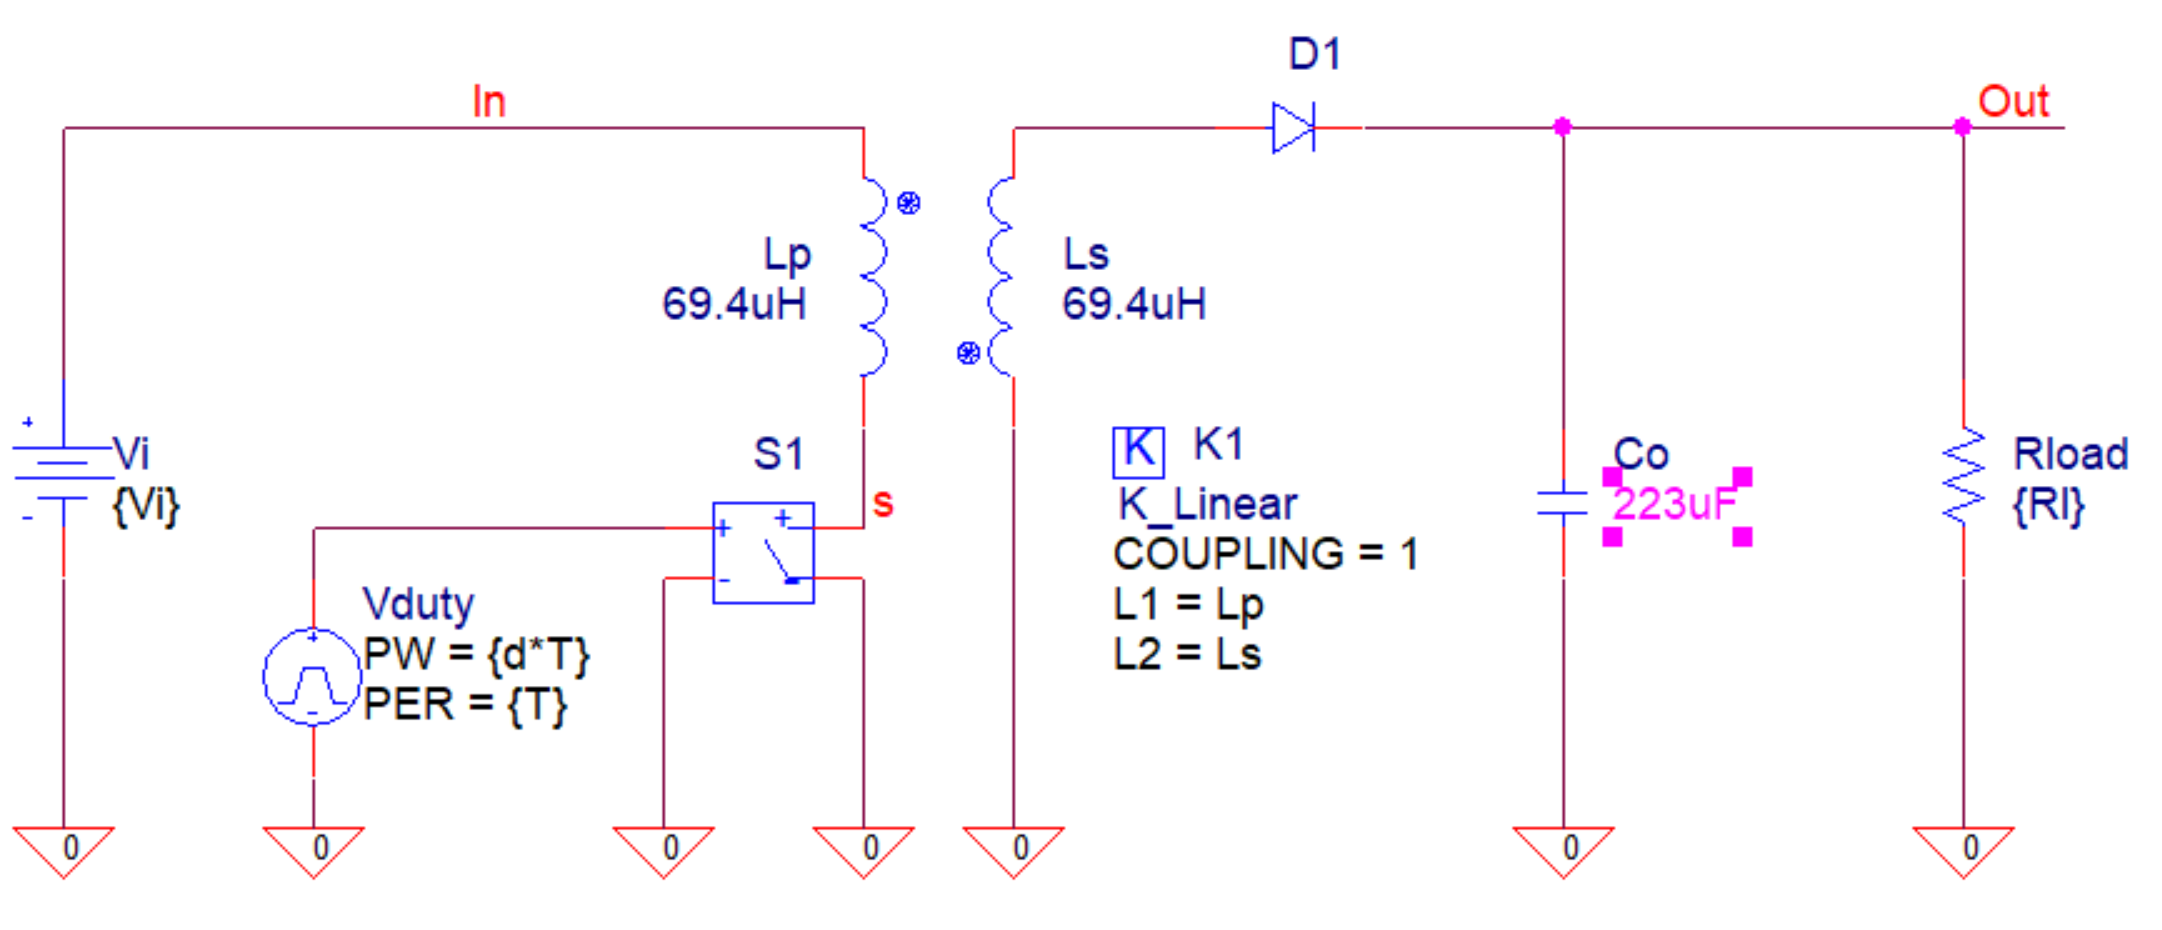
\includegraphics[max width=0.7\linewidth]{/tex/smps/billeder/flyback_ideal_diagram.PNG}
	\caption{Ideelt flyback kredsløb}
	\label{fig:ideal_flyback_diagram}
\end{figure}

Der er to scenarier der er relevante at kigge på, ved en indgangsspænding på $26V$, samt ved en indgangsspænding på $100V$. Først kigges der på udgangen af converteren, for at kontrollere udgangsstrømmen og -spændingen. På figur~\ref{fig:26V_ideal_output} ses både outputstrømmen (rød) og outputspændingen (grøn), med en inputspænding på 26V. Her ses det at spændingen ligger sig omkring $21V$ og strømmen ligger sig omkring $2.5A$, hvilket var kravet til converteren. Derudover aflæses ripplespændingen til ca. $50mV$, hvilket er overholder kravet for ripplespændingen. 

\begin{figure}[H]
	\center
	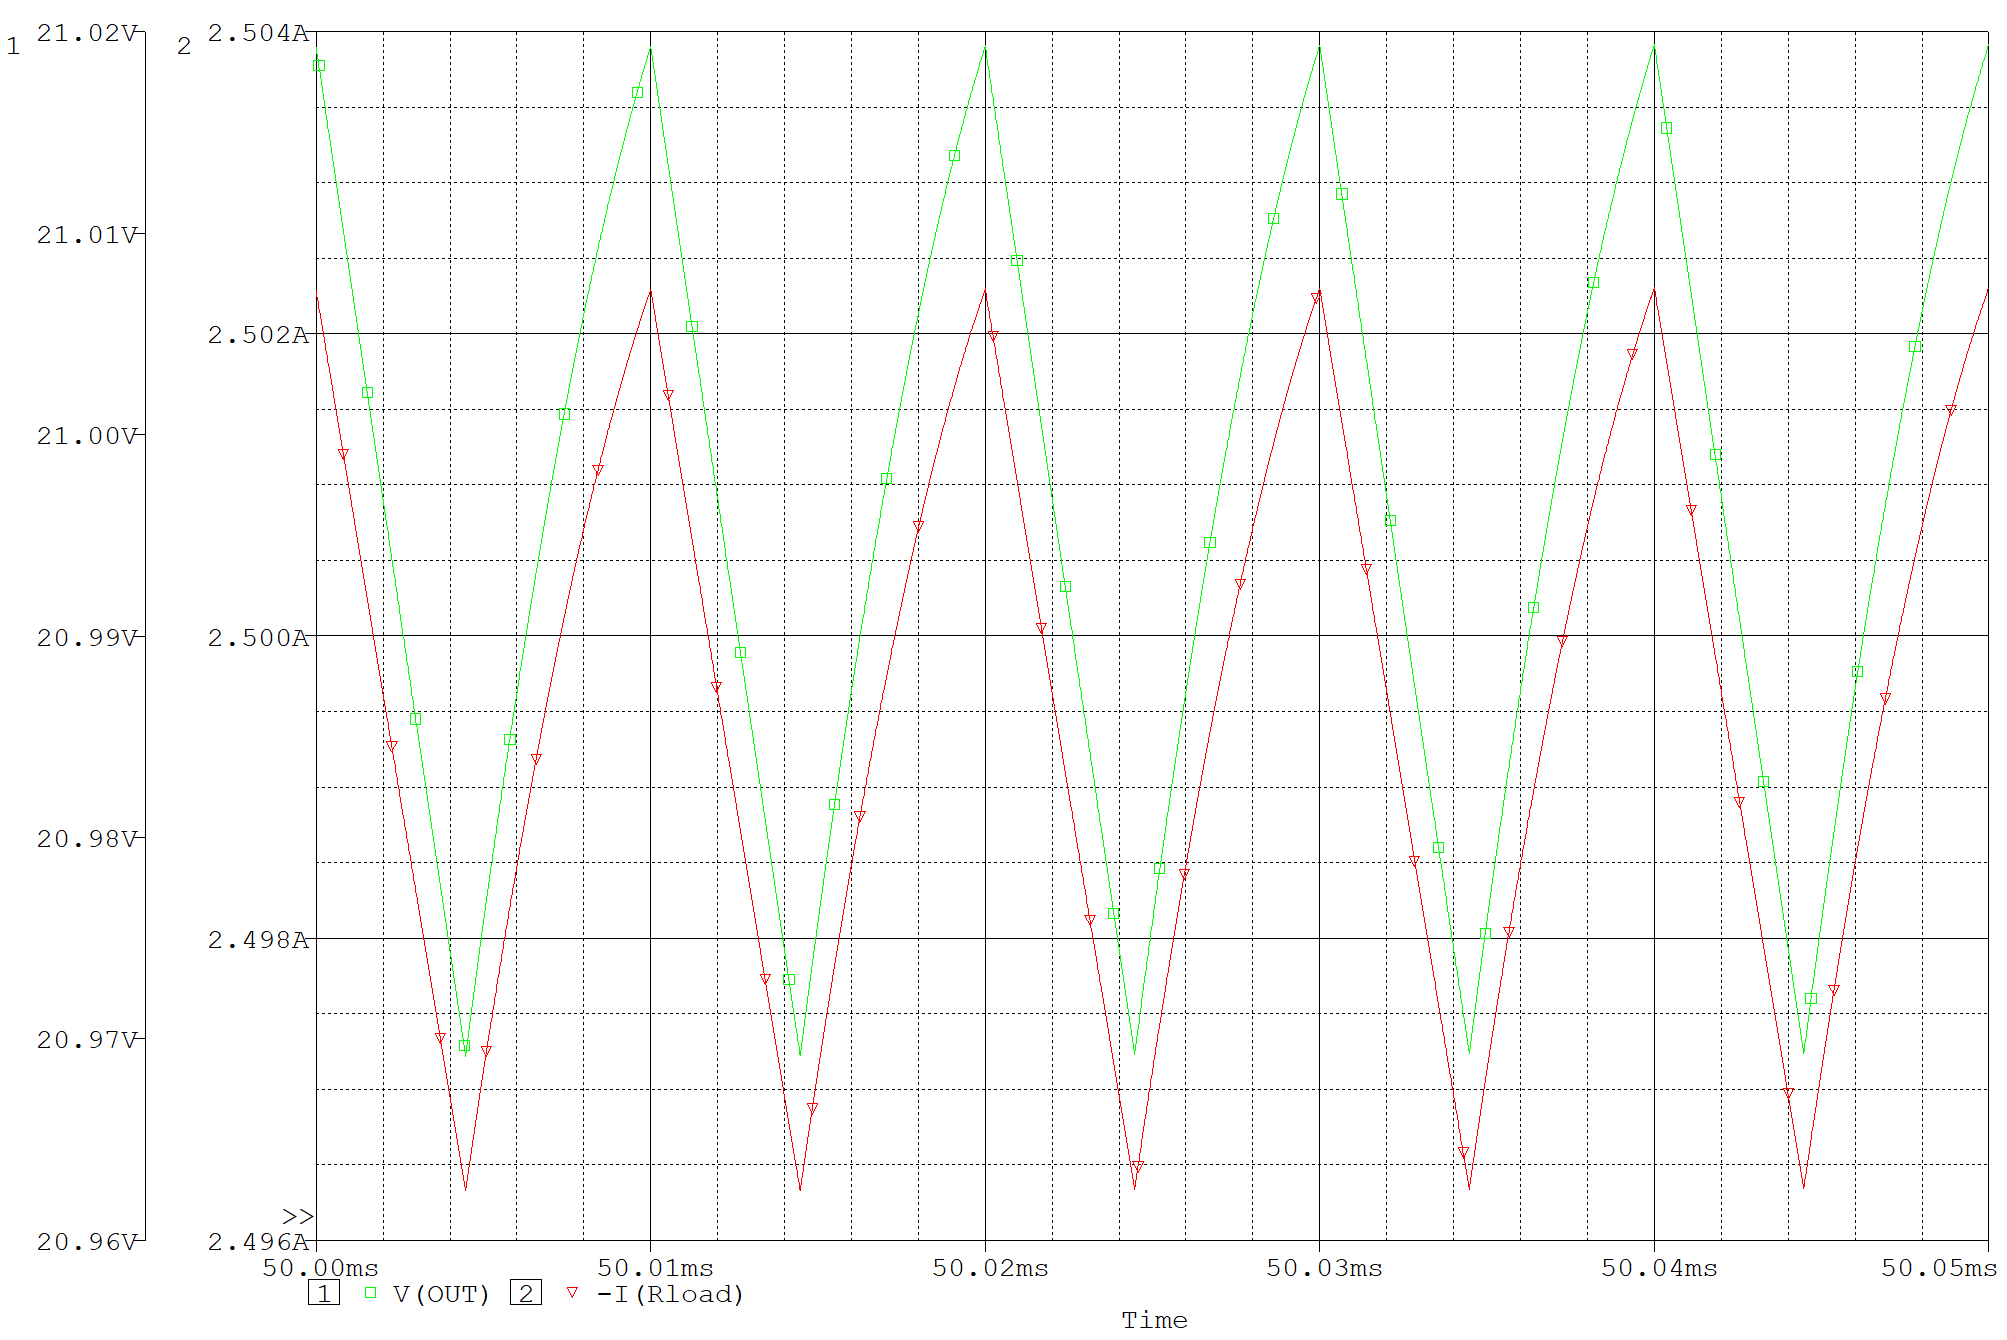
\includegraphics[max width=0.7\linewidth]{/tex/smps/billeder/26V_output.PNG}
	\caption{Converter output - ved 26V input}
	\label{fig:26V_ideal_output}
\end{figure}

\noindent På figur~\ref{fig:100V_ideal_output} ses det samme billede, ved 100V inputspænding. Da converterens duty-cycle er faldet, falder ripple-spændingen også. Den aflæses til ca. $20mV$. 
%TODO Forklar mærkelig kurve form.

\begin{figure}[H]
	\center
	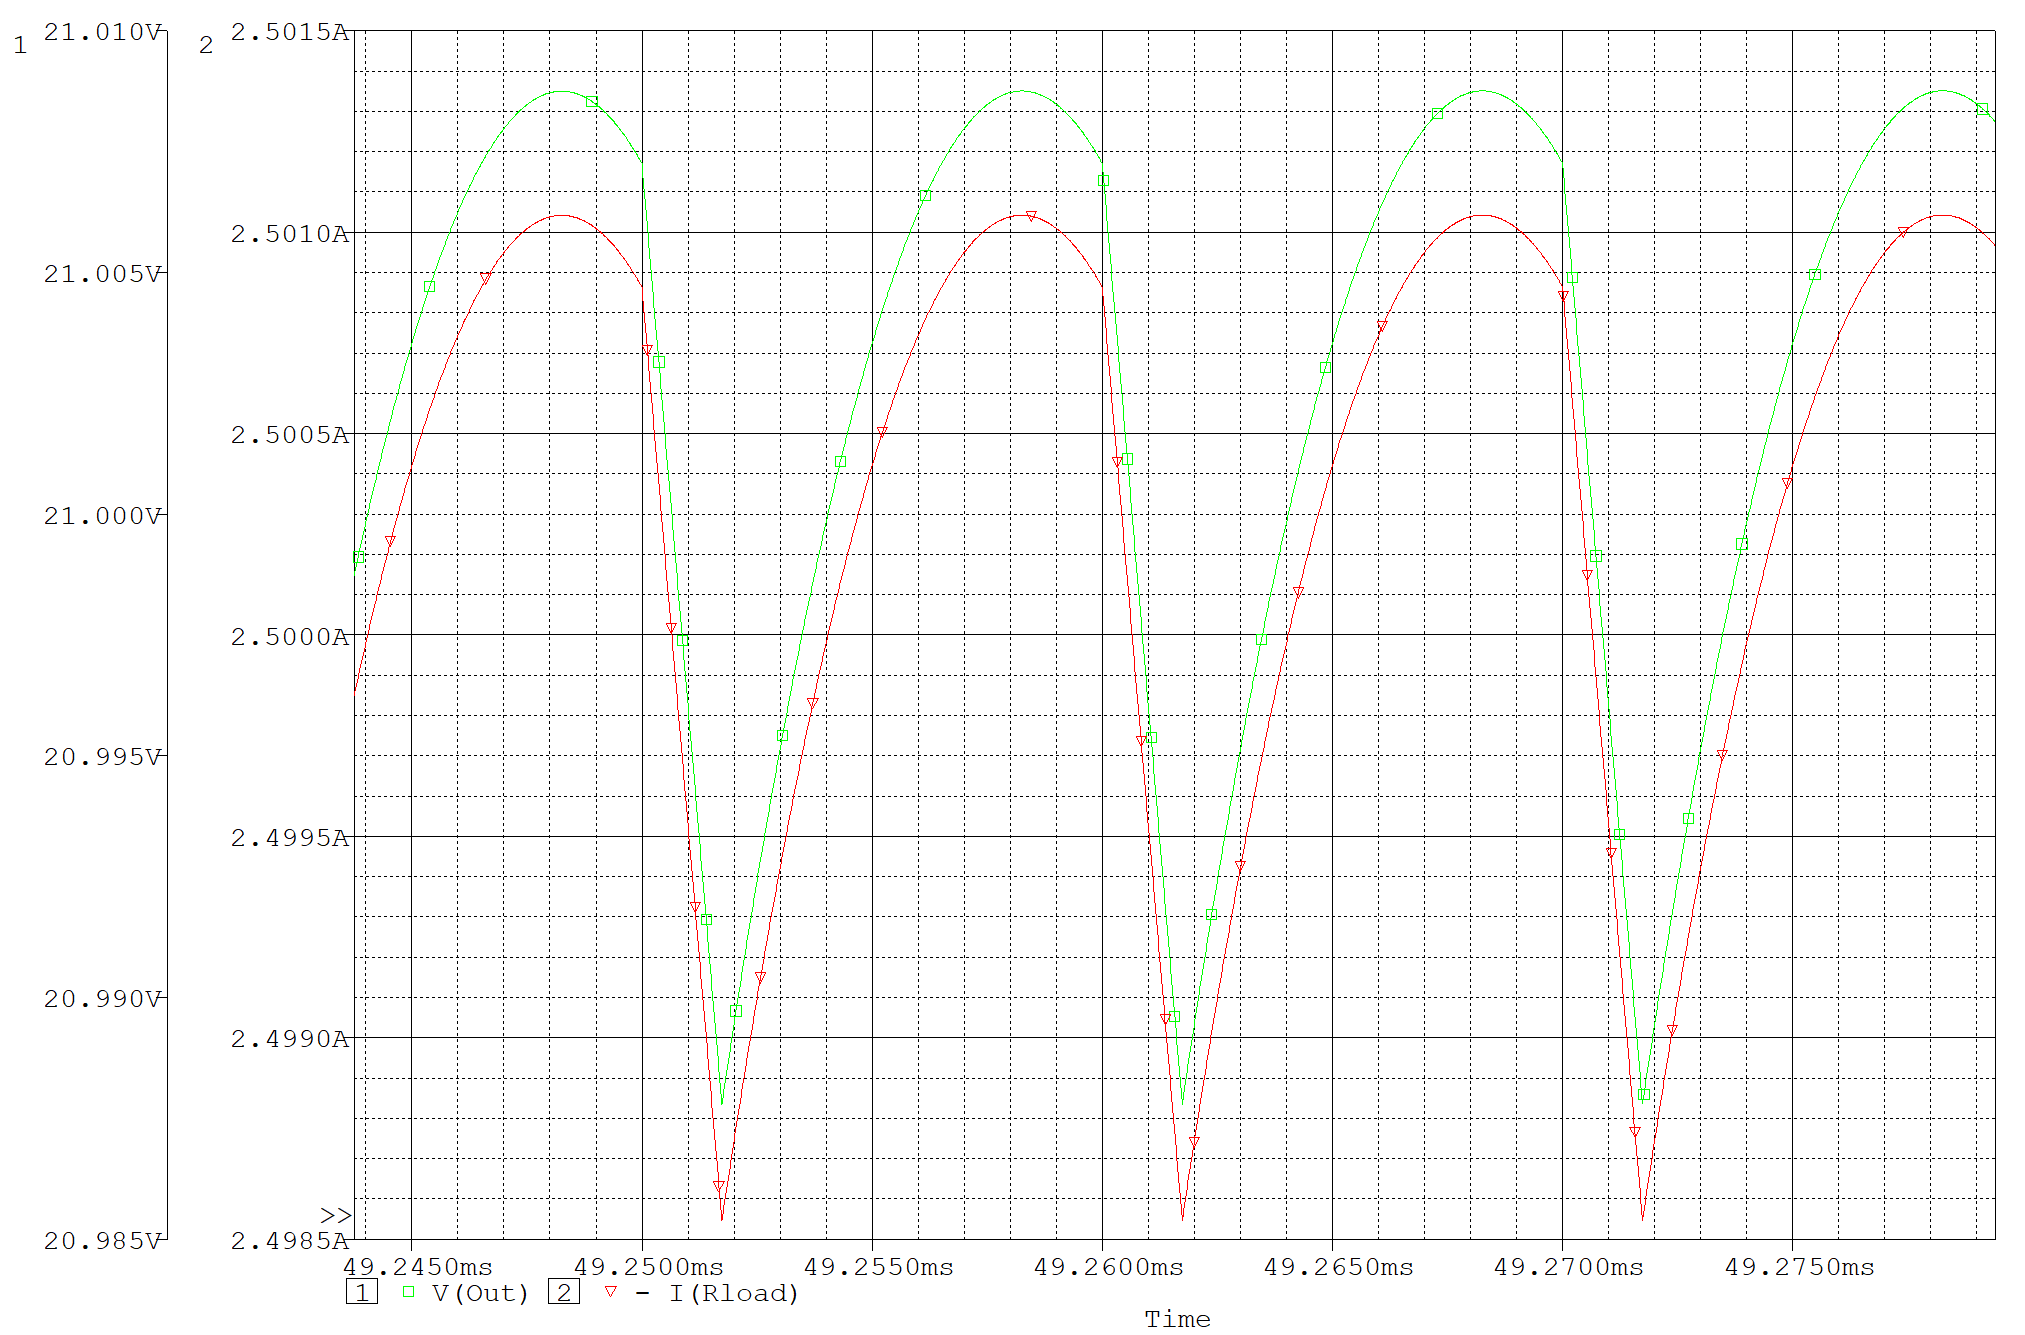
\includegraphics[max width=0.7\linewidth]{/tex/smps/billeder/100V_output.PNG}
	\caption{Converter output - ved 100V input}
	\label{fig:100V_ideal_output}
\end{figure}

\noindent I tabel~\ref{tab:result_ideal_converter} ses resultaterne for analyse(A) og simulering(S), af den ideelle converter. Ripple- og peakstrømmene er aflæst ud fra figur~\ref{fig:26V_transformer_current} og \ref{fig:100V_transformer_current}. RMS-strømmene findes ved, at bruge RMS-funktionen i p-spice. Derudover kan det konstateres at converteren operer i CCM, da transformatorstrømmen ikke når at aflade helt. Se figur~\ref{fig:CCM_transformer_current}. 

\begin{table}[H] 			
	\centering
	\begin{tabularx}{\textwidth}{|X|c|c|c|c|c|c|c|c|}
		\hline
		\textbf{Indgangs-spænding} & \multicolumn{2}{|X|}{\textbf{Ripplestrøm}} & \multicolumn{2}{|X|}{\textbf{Peakstrøm}} & \multicolumn{2}{|X|}{\textbf{RMS-strøm i primær}} & \multicolumn{2}{|X|}{\textbf{RMS-strøm i sekundær}} \\ \hline
		& A & S & A & S & A & S & A & S \\ \hline
		$26V$ & $1.2A$ & $1.2A$ & $5.1A$ & $5.1A$ & $3.0A$ & $3.0A$ & $3.4A$ & $3.4A$ \\ \hline 
		$100V$ & $1.8A$ & $1.8A$ & $3.9A$ & $3.9A$ & $1.3A$ & $1.3A$ & $2.8A$ & $2.8A$ \\ \hline
	\end{tabularx}
	\caption{Resultater for analyse og simulering af ideel flyback converter}
	\label{tab:result_ideal_converter}
\end{table}

\begin{figure}[H]
	\center
	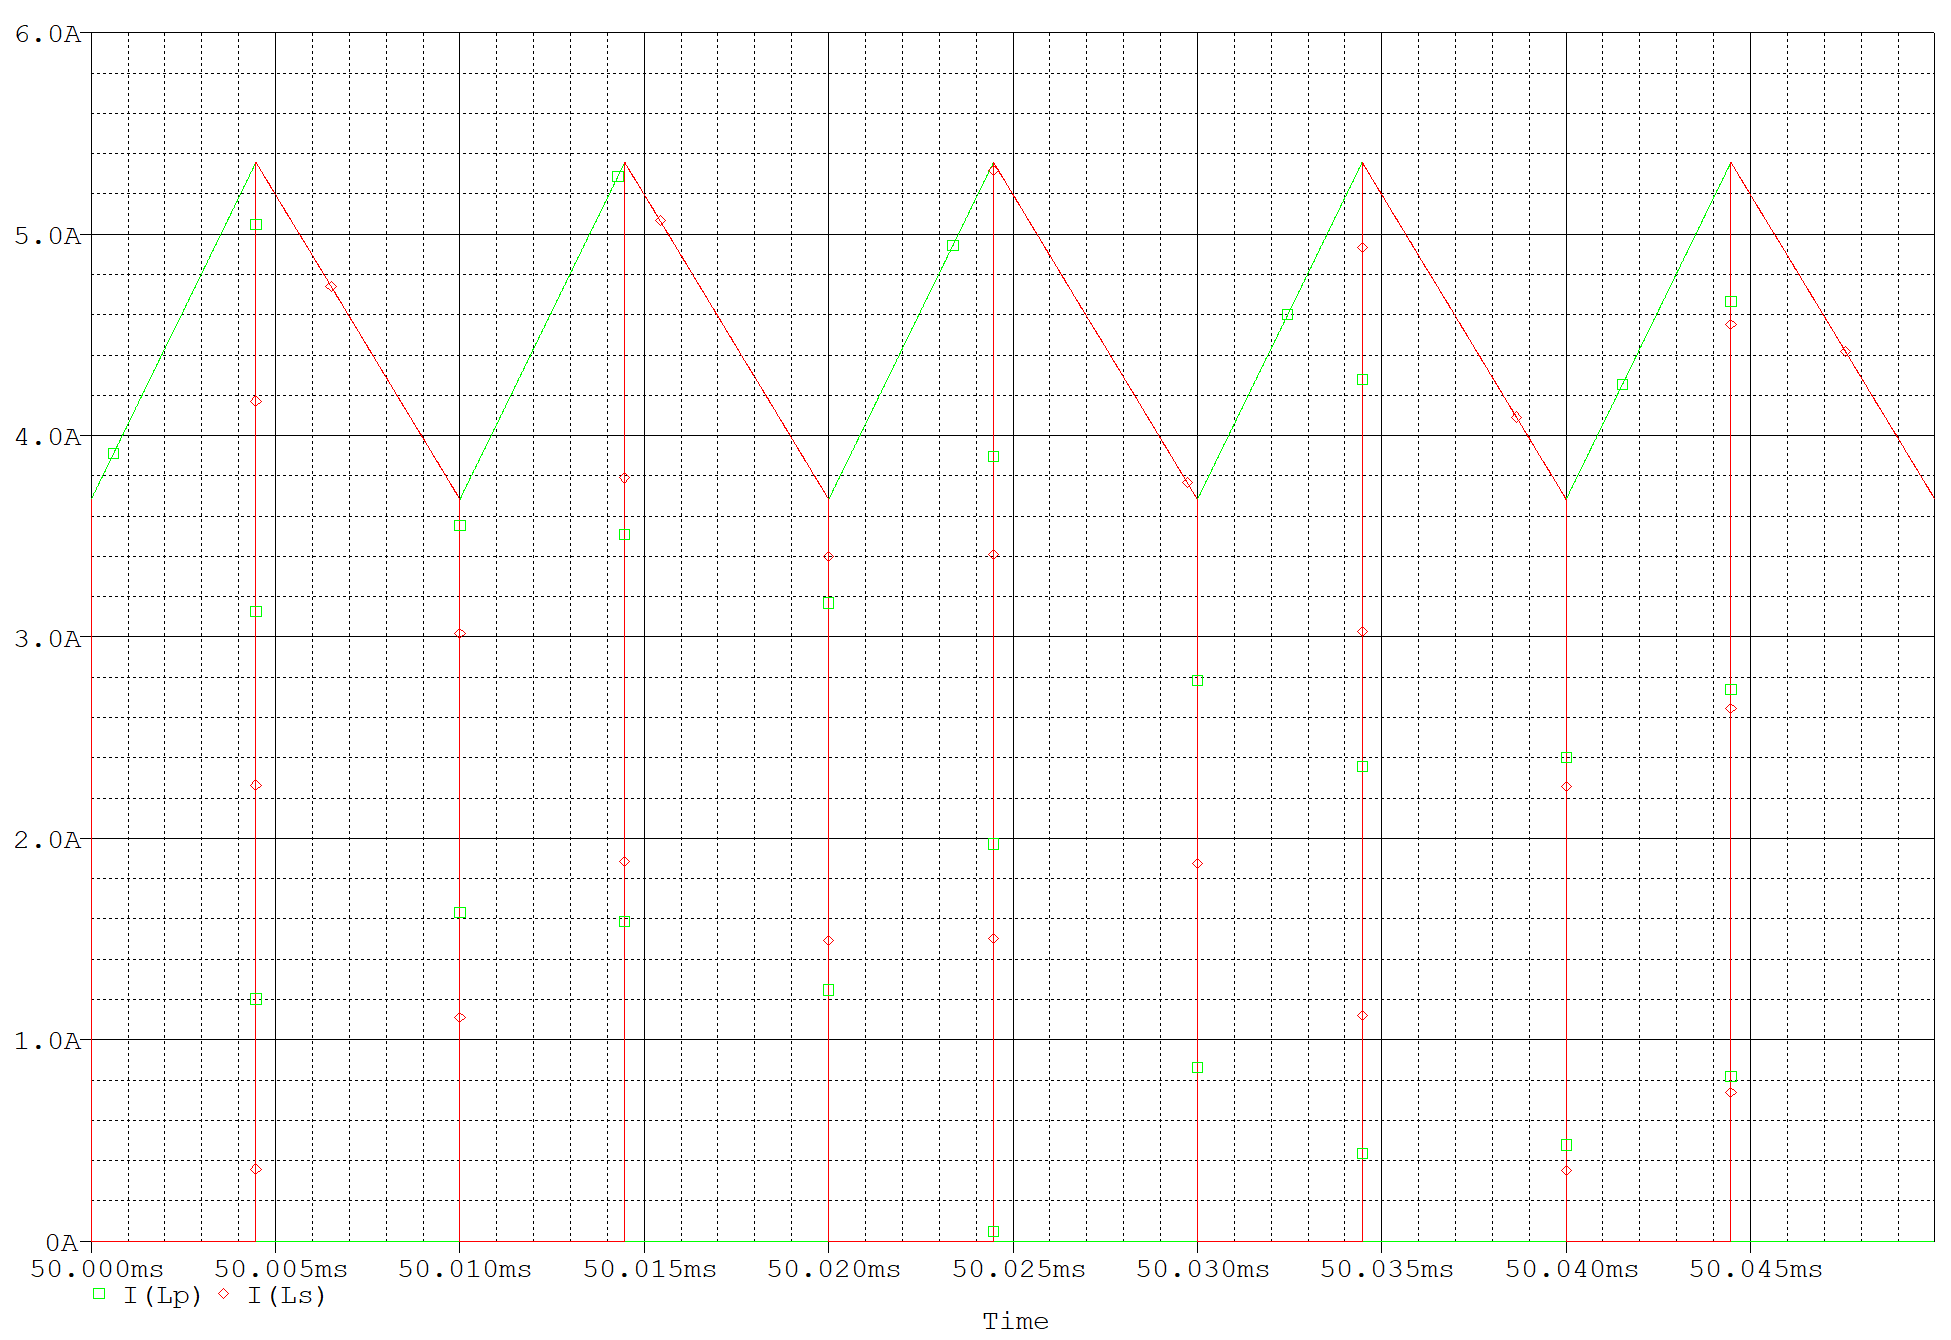
\includegraphics[max width=0.7\linewidth]{/tex/smps/billeder/26V_transformer_current.PNG}
	\caption{Transformator strømme - ved 26V input}
	\label{fig:26V_transformer_current}
\end{figure}

\begin{figure}[H]
	\center
	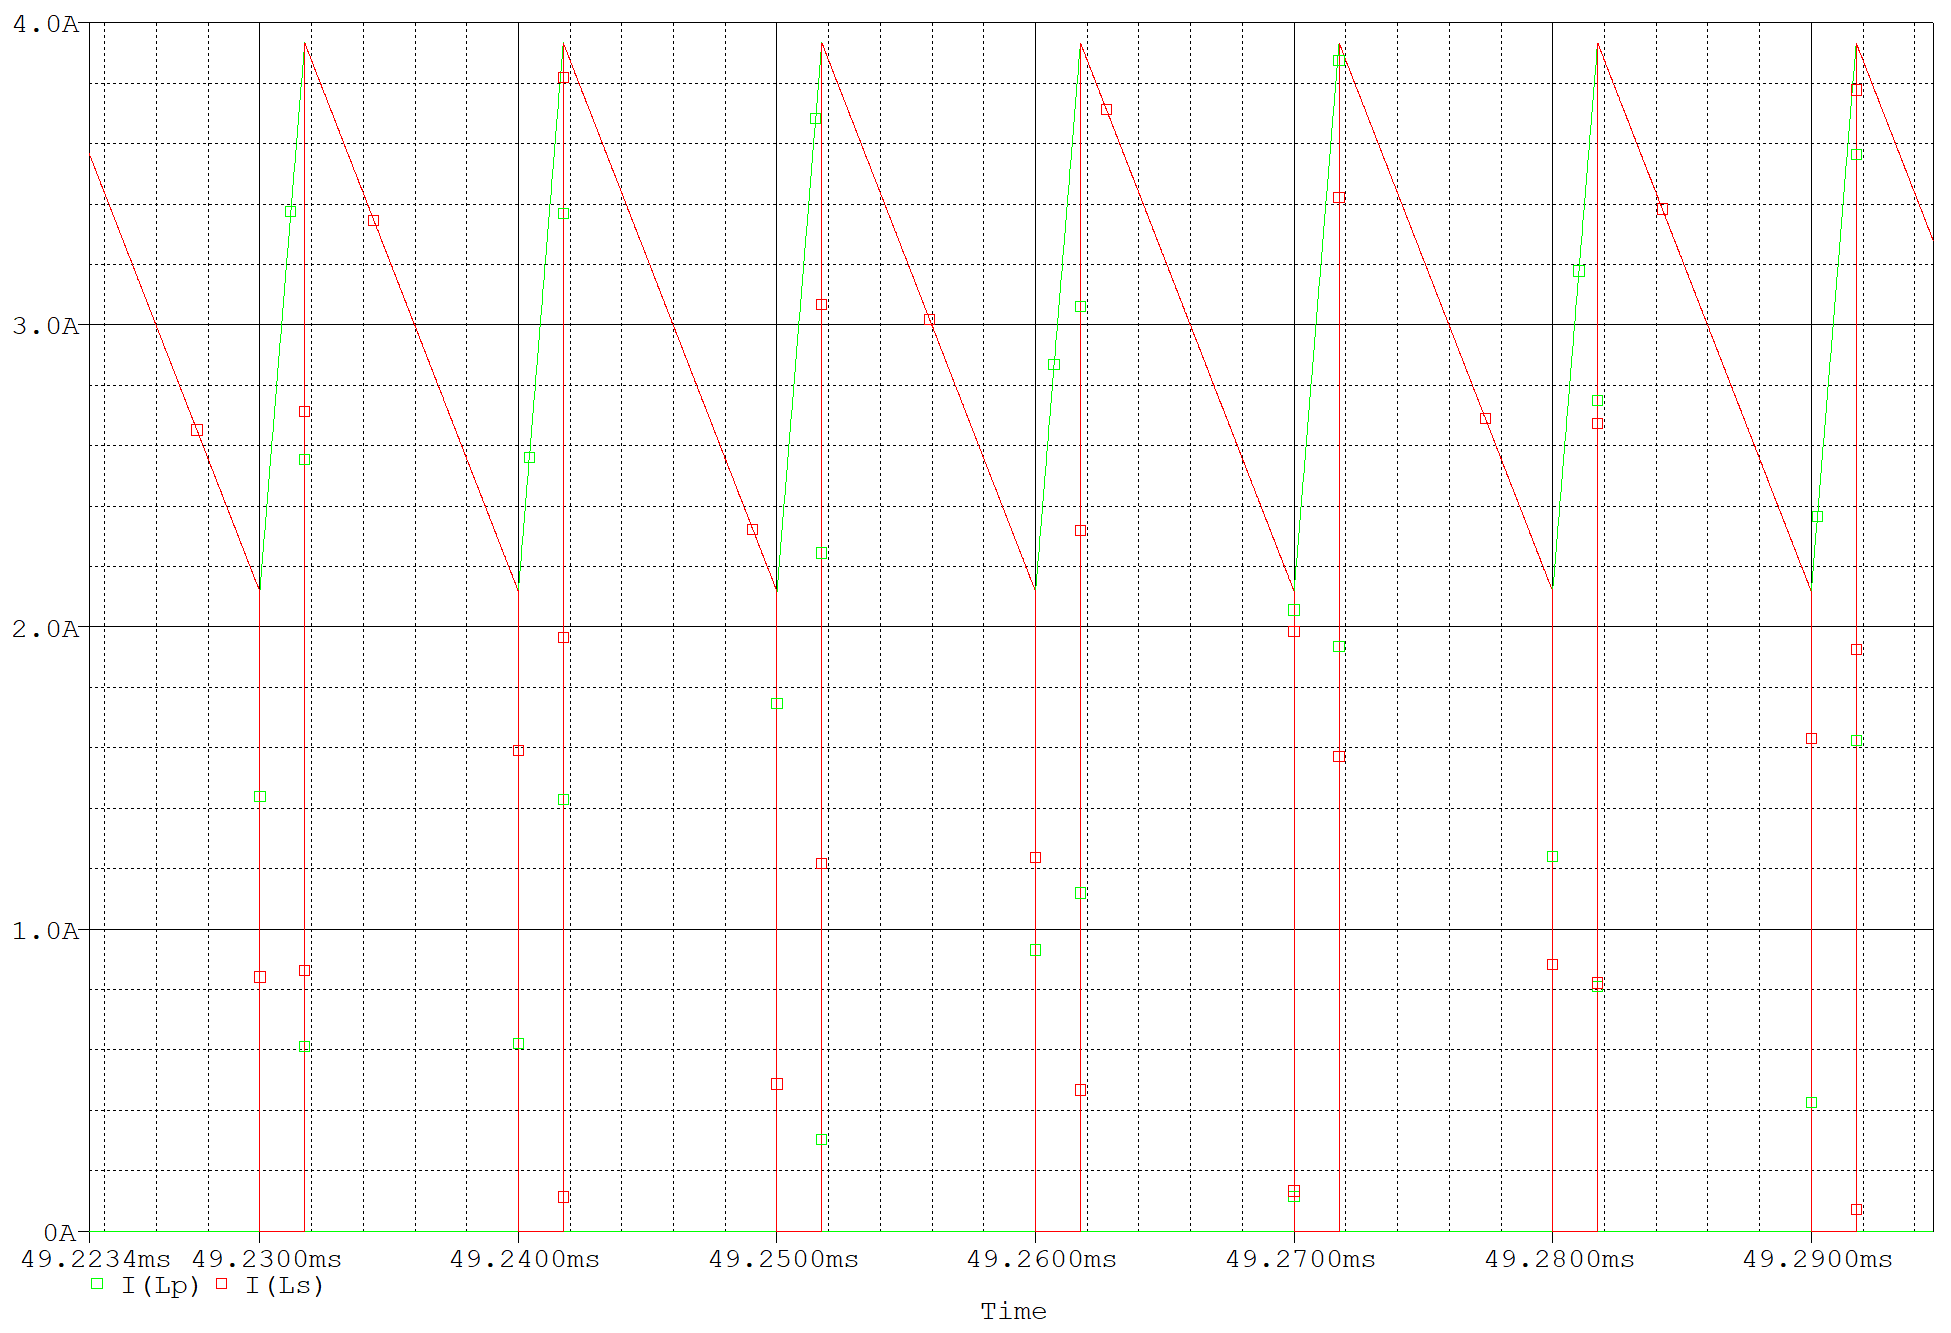
\includegraphics[max width=0.7\linewidth]{/tex/smps/billeder/100V_transformer_current.PNG}
	\caption{Transformator strømme - ved 100V input}
	\label{fig:100V_transformer_current}
\end{figure}



